% !TeX TS-program = xelatex -synctex=1 -interaction=nonstopmode -shell-escape -output-directory=build %.tex
\documentclass[aspectratio=169]{beamer}

% All my packages are specified and set up in include/format:
\usepackage{include/format}

\title{Arduino IDE}
\subtitle{ESP32 guide}

\author{Jacob Bechmann Pedersen}
\institute{Bechmann Engineering ApS}
\date{\today}

%% Reference settings:
\renewcommand{\figurename}{Figur}
\renewcommand{\tablename}{Tabel}
\renewcommand{\refname}{Referenceliste}
\renewcommand{\contentsname}{Indhold}
\renewcommand{\listfigurename}{Figurliste}
\renewcommand{\listtablename}{Tabelliste}
\renewcommand{\lstlistlistingname}{Kodeliste}

\begin{document}

\begin{frame}
	\titlepage
\end{frame}

\begin{frame}{Indhold}
		\begin{fitBox}
			\tableofcontents{}
		\end{fitBox}
\end{frame}

\section{Ressourcer}
\begin{frame}{Ressourcer}
	\begin{textBox}
	Nogle nyttige links:
		\begin{itemize}
			\item \url{https://github.com/iakop/IoT-Crashcourse}
			\begin{itemize}
				\item Præsentation og kode til denne workshop
			\end{itemize}
			\item \url{https://www.arduino.cc/en/software\#legacy-ide-18x}
			\begin{itemize}
				\item Download af Arduino IDE \tthigh{1.8.X}
				\begin{itemize}
					\item \ttwarn{IKKE 2.X.X}
				\end{itemize}
				\item Windows version at downloade: \tthigh{Win 7 or newer} 
				\begin{itemize}
					\item \ttwarn{IKKE Windows app Win 8.1 or 10}
					\item Dvs. \ttwarn{undgå} dette logo: (
\includegraphics[height=8pt, keepaspectratio=true]{assets/pictures/windows-get.png})
				\end{itemize}
				\item Mac OS X version at downloade: \tthigh{10.10 or newer} 
				\item Linux version at downloade: \tthigh{64 bits/Det ved du selv}\color{arduinoBlue}😜%\emojifont{😜}
			\end{itemize}
			\item \url{https://www.arduino.cc/en/reference}
			\begin{itemize}
				\item Reference for keywords i Arduino
			\end{itemize}
		\end{itemize}
	\end{textBox}
\end{frame}

\section{Setup af ESP32 på Arduino IDE}
\begin{frame}
	\sectiontitle{assets/pictures/arduino-ide.png}{\insertsectionhead}
\end{frame}

\subsection{Setup Arduino IDE}
\begin{frame}{Setup Arduino IDE}
\begin{columns}
	\begin{column}{0.5\textwidth}
		\begin{figure}
  			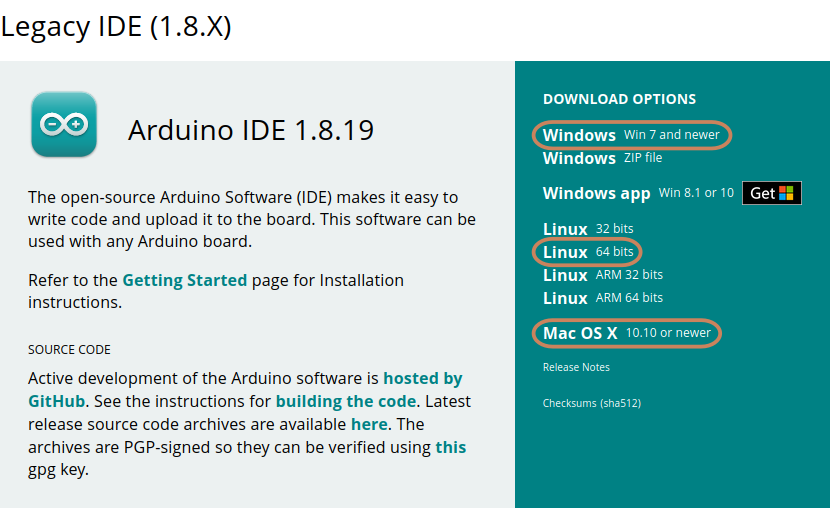
\includegraphics[width=\textwidth,keepaspectratio=true]{assets/pictures/arduino-versions.png}
  			\caption{\tthigh{Arduino Legacy IDE (1.8.X)}, versionen der bliver benyttet i denne workshop. Versionerne highlighted er de understøttede versioner}
  			\label{fig:arduino-versions}
		\end{figure}
	\end{column}
	\begin{column}{0.5\textwidth}
		\begin{textBox}
			\begin{itemize}
				\item Download Arduino IDE \tthigh{1.8.X} fra linket:
				\begin{itemize}
					 \item \small\url{https://www.arduino.cc/en/software\#legacy-ide-18x}
				\end{itemize}
				\begin{itemize}
					\item \ttwarn{IKKE 2.X.X}
					\item Windows:
					\begin{itemize}
						\item  \tthigh{Win 7 or newer} 
						\item \ttwarn{IKKE Windows app Win 8.1 or 10}
						\item Dvs. \ttwarn{undgå} dette logo: (
\includegraphics[height=8pt, keepaspectratio=true]{assets/pictures/windows-get.png})
					\end{itemize}
					\item Mac OS X:
					\begin{itemize}
						\item \tthigh{10.10 or newer}
					\end{itemize}
					\item Linux:
					\begin{itemize}
						\item \tthigh{64 bits/Det ved du selv}\color{arduinoBlue}😜%\emojifont{😜}
					\end{itemize}
				\end{itemize}
			\end{itemize}
		\end{textBox}
	\end{column}
\end{columns}
\end{frame}

\begin{frame}{Setup Arduino IDE}
\begin{columns}
	\begin{column}{0.5\textwidth}
		\begin{textBox}
			\begin{itemize}
				\item Der vil komme en donationsside
				\item Bare vælg "\tthigh{Just Download}"
			\end{itemize}
		\end{textBox}
	\end{column}
	\begin{column}{0.5\textwidth}
		\begin{figure}
  			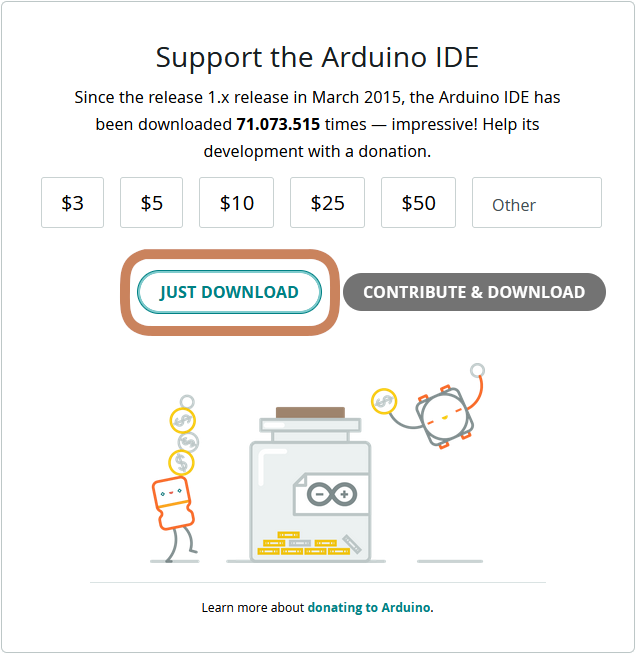
\includegraphics[height=0.6\textheight]{assets/pictures/just-download.png}
  			\caption{Donationssiden for Arduino, blot vælg "\tthigh{Just Download}" for at downloade uden at donere}
  			\label{fig:just-download}
		\end{figure}
	\end{column}
\end{columns}
\end{frame}

\begin{frame}{Setup Arduino IDE}
\begin{columns}
	\begin{column}{0.5\textwidth}
		\begin{figure}
  			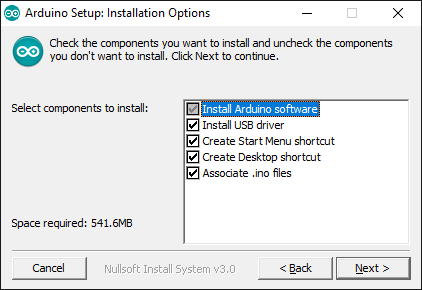
\includegraphics[height=0.6\textheight,keepaspectratio=true]{assets/pictures/install-all.png}
  			\caption{Installationsdialog på Windows. Alle bokse skal mærkes med ✔️}
  			\label{fig:install-all}
		\end{figure}
	\end{column}
	\begin{column}{0.5\textwidth}
		\begin{textBox}
			\begin{itemize}
				\item Ved installation, tilvælg og sig "\tthigh{Yes}" til alle drivers der installeres
			\end{itemize}
		\end{textBox}
	\end{column}
\end{columns}
\end{frame}

\begin{frame}{Setup Arduino IDE}
\begin{columns}
	\begin{column}{0.5\textwidth}
		\begin{textBox}
			\begin{itemize}
				\item Ved installation, tilvælg og sig "\tthigh{Yes}" til alle drivers der installeres
				\item Efter installation åbn \tthigh{Arduino IDE} - hvis vinduet åbner, er installationen lykkedes!
				\item Bemærk knapperne i toppen. De væsentligste:
				\begin{itemize}
					\item \includesvg[height=12pt, keepaspectratio=true]{assets/svg/ide-verify.svg} Verify
					\begin{itemize}
						\item Kompilerer koden, og outputter evt. fejl nederst i vinduet
					\end{itemize}
					\item \includesvg[height=12pt, keepaspectratio=true]{assets/svg/ide-upload.svg} Upload
					\begin{itemize}
						\item Kompilerer koden, og uploader den til det tilsluttede board
					\end{itemize}
					\item \includesvg[height=12pt, keepaspectratio=true]{assets/svg/ide-serial.svg} Serial Monitor
					\begin{itemize}
						\item Åbner et vindue til seriel kommunikation mellem board og computer
					\end{itemize}
				\end{itemize}
			\end{itemize}
		\end{textBox}
	\end{column}
	\begin{column}{0.5\textwidth}
		\begin{figure}
  			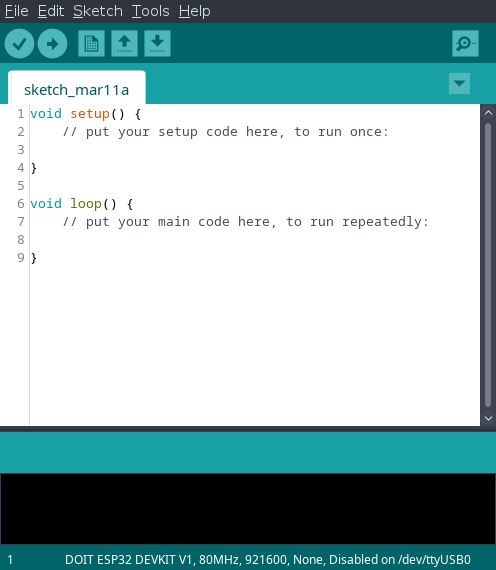
\includegraphics[height=0.6\textheight,keepaspectratio=true]{assets/pictures/arduino-ide.png}
  			\caption{Arduino IDE 1.8.19 default sketch ved første opstart}
  			\label{fig:arduino-ide}
		\end{figure}
	\end{column}
\end{columns}
\end{frame}

\subsection{Board Definitions}
\begin{frame}{Board Definitions}
\begin{columns}
	\begin{column}{0.5\textwidth}
		\begin{figure}
  			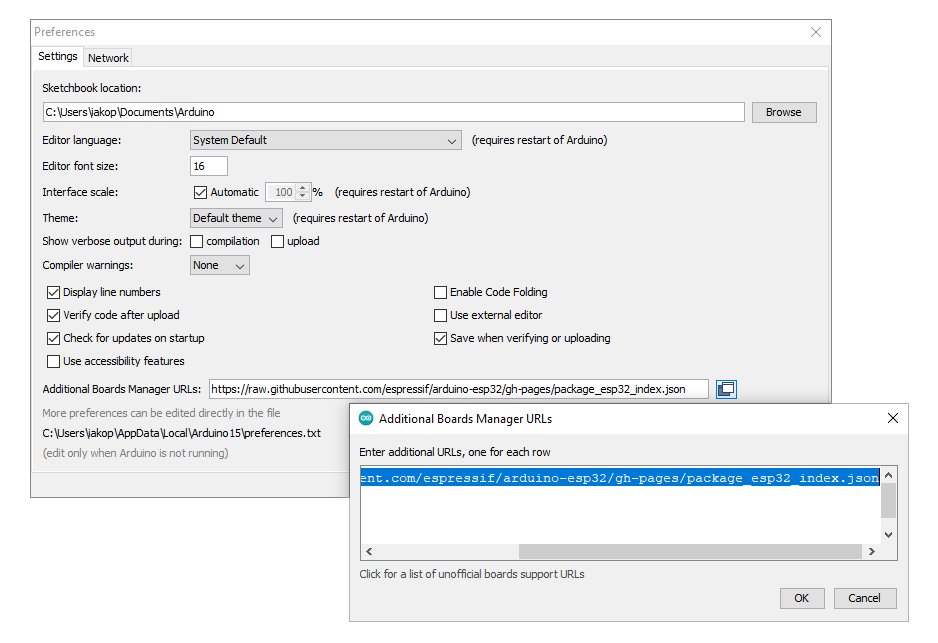
\includegraphics[width=\textwidth]{assets/pictures/boardsmanager.png}
  			\caption{Preferences manager i Arduino IDE 1.8.19}
  			\label{fig:boardsmanager}
		\end{figure}
	\end{column}
	\begin{column}{0.5\textwidth}
		\begin{textBox}
			\begin{itemize}
				\item I Arduino IDE:
				\begin{itemize}
					 \item "\tthigh{File} > \tthigh{Preferences}"
				\end{itemize}
				\item Indsæt URL i "\tthigh{Additional Boards Manager URLs}":
				\begin{itemize}
					 \item \tiny\url{https://raw.githubusercontent.com/espressif/arduino-esp32/gh-pages/package_esp32_index.json}
				\end{itemize}
				\item \tthigh{OBS}: Tjek og fjern eventuelle spaces i det copy-pastede URL
			\end{itemize}
		\end{textBox}
	\end{column}
\end{columns}
\end{frame}

\begin{frame}{Board Definitions}
\begin{columns}
	\begin{column}{0.5\textwidth}
		\begin{textBox}
			\begin{itemize}
				\item Under "\tthigh{Tools} > \tthigh{Board} > \tthigh{Boards Manager}"
				\item Søg efter "\tthigh{ESP32}" og tryk "\tthigh{Install}" ud fra den seneste version
				\begin{itemize}
					 \item Der skal hentes omkring 250MB, så det tager lidt tid
				\end{itemize}
			\end{itemize}
		\end{textBox}
	\end{column}
	\begin{column}{0.5\textwidth}
		\begin{figure}
  			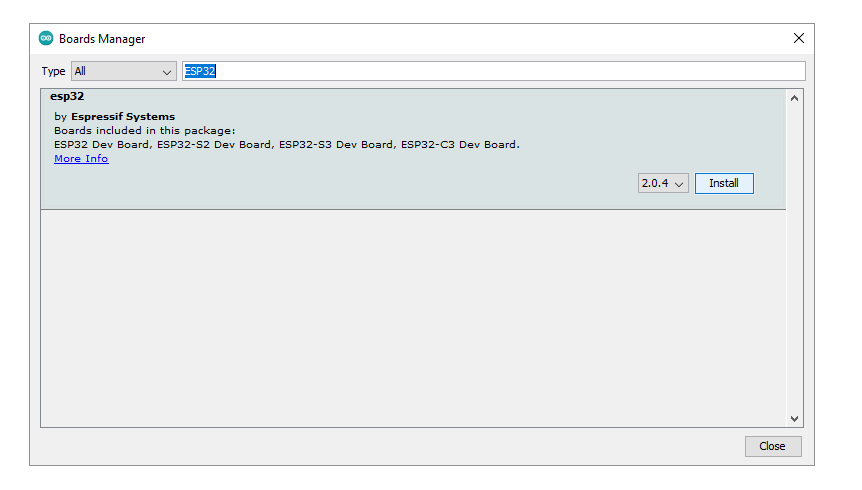
\includegraphics[width=\textwidth]{assets/pictures/boardsmanager2.png}
  			\caption{Boards Manager, her kan board definitions (beskrivelse af hardware og programmeringsværktøjer) hentes fra de kendte board manager URLs i Arduino IDE}
  			\label{fig:boardsmanager2}
		\end{figure}
	\end{column}
\end{columns}
\end{frame}

\subsection{Libraries og Tools}
\begin{frame}{Libraries og Tools}
\begin{columns}
	\begin{column}{0.5\textwidth}
		\begin{figure}
  			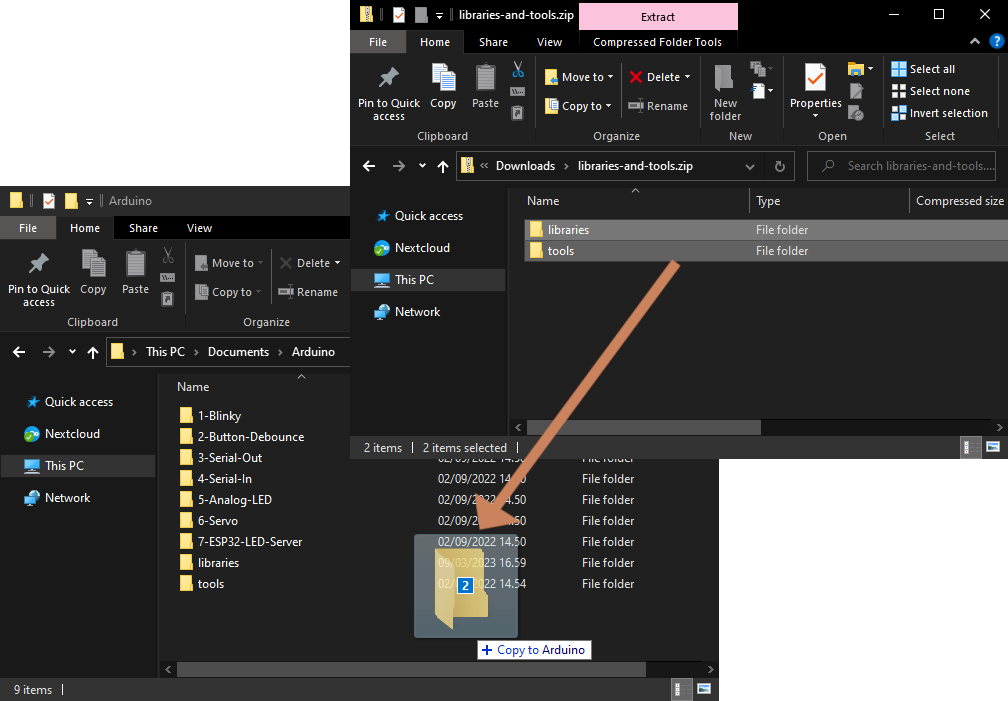
\includegraphics[width=\textwidth]{assets/pictures/extract-to-arduino.png}
  			\caption{Arkivet indeholder to mapper, "\tthigh{libraries}" og "\tthigh{tools}" som Arduino bruger til at holde hhv. libraries og værktøjer til IDE'et i sin default mappe under "\tthigh{Documents}/ \tthigh{Arduino}"}
  			\label{fig:libraries-and-tools}
		\end{figure}
	\end{column}
	\begin{column}{0.5\textwidth}
		\begin{textBox}
			\begin{itemize}
				\item Download arkivet "\tthigh{libraries-and-tools.zip}" fra linket:
				\begin{itemize}
					\item \tiny\url{https://raw.githubusercontent.com/iakop/IoT-Crashcourse/master/extra/libraries-and-tools.zip}
				\end{itemize}
				\item Udpak indholdet i din PC's "\tthigh{Documents}/ \tthigh{Arduino}" folder
				\item Den skulle nu indeholde en mappe ved navn "\tthigh{libraries}" og en ved navn "\tthigh{tools}"
			\end{itemize}
		\end{textBox}
	\end{column}
\end{columns}
\end{frame}


\begin{frame}{Libraries og Tools}
\begin{columns}
	\begin{column}{0.5\textwidth}
		\begin{textBox}
			\begin{itemize}
				\item For at tjekke at de nødvendige libraries er installeret, genstart Arduino IDE, åbn "\tthigh{Tools} > \tthigh{Manage Libraries...}"
				\item Installerede libraries kan tjekkes i øverste venstre hjørne under "\tthigh{Type}": "\tthigh{Installed}"
				\item Disse libraries bør nu alle være tilstede:
				\begin{itemize}
					\item \tthigh{ArduinoJson}
					\item \tthigh{Adafruit Unified Sensor}
					\item \tthigh{DHT sensor library}
					\item \tthigh{MQTT}
				\end{itemize}
				\item \tthigh{ESPAsyncWebServer} og \tthigh{AsyncTCP} er ikke tracket af Arduino IDE, men ligger i "\tthigh{libraries}" mappen
			\end{itemize}
		\end{textBox}
	\end{column}
	\begin{column}{0.5\textwidth}
		\begin{figure}
  			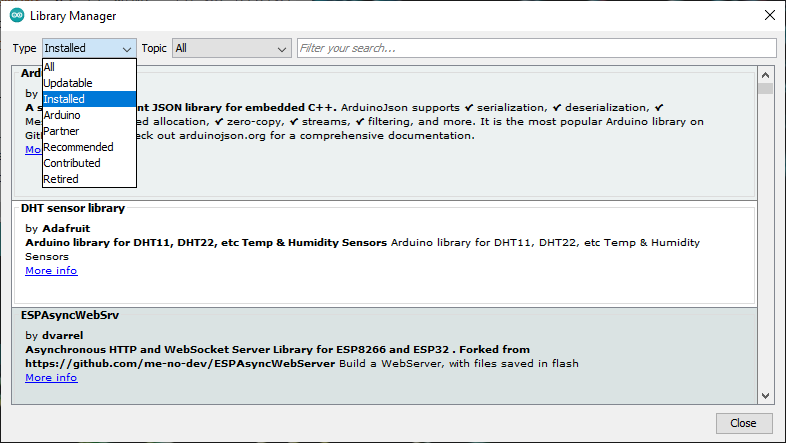
\includegraphics[width=\textwidth]{assets/pictures/librarymanager-installed.png}
  			\caption{"\tthigh{Library Manager}" kan bruges til at installere nye libraries der understøttes af Arduino platformen. Den kan også bruges til at se de installerede libraries eller opdatere dem}
  			\label{fig:librarymanager-installed}
  		\end{figure}
	\end{column}
\end{columns}
\end{frame}

\begin{frame}{Libraries og Tools}
\begin{columns}
	\begin{column}{0.5\textwidth}
			\begin{figure}
  					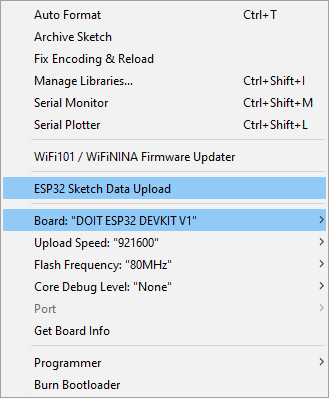
\includegraphics[width=0.5\textwidth]{assets/pictures/sketch-data-and-board.png}
  					\caption{Værktøjet "\tthigh{ESP32 Sketch Data Upload}" bruges bl.a. til at lægge .html indhold på ESP32's filsystem. Board definitionen "\tthigh{DOIT ESP32 DEVKIT V1}" sikrer, der bliver uploadet kode i det rigtige format}
  					\label{fig:sketch-data-and-board}
  			\end{figure}
	\end{column}
	\begin{column}{0.5\textwidth}
		\begin{textBox}
			\begin{itemize}
				\item For at tjekke at om de rette tools, samt Board Definitions er installeret, åbn "\tthigh{Boards}"
				\item I menuen skal feltet "\tthigh{ESP32 Sketch Data Upload}" være tilgængeligt
				\item Under feltet "\tthigh{Board:}" skal man kunne vælge "\tthigh{Board} > \tthigh{ESP32 Arduino} > \tthigh{DOIT ESP32 DEVKIT V1}"
			\end{itemize}
		\end{textBox}
	\end{column}
\end{columns}
\end{frame}

\section{Upload til ESP32}
\begin{frame}
	\sectiontitle{assets/pictures/arduino-ide.png}{\insertsectionhead}
\end{frame}

\subsection{Åbning af sketch}
\begin{frame}{Åbning af sketch}
\begin{columns}

	\begin{column}{0.5\textwidth}
		\begin{figure}
  			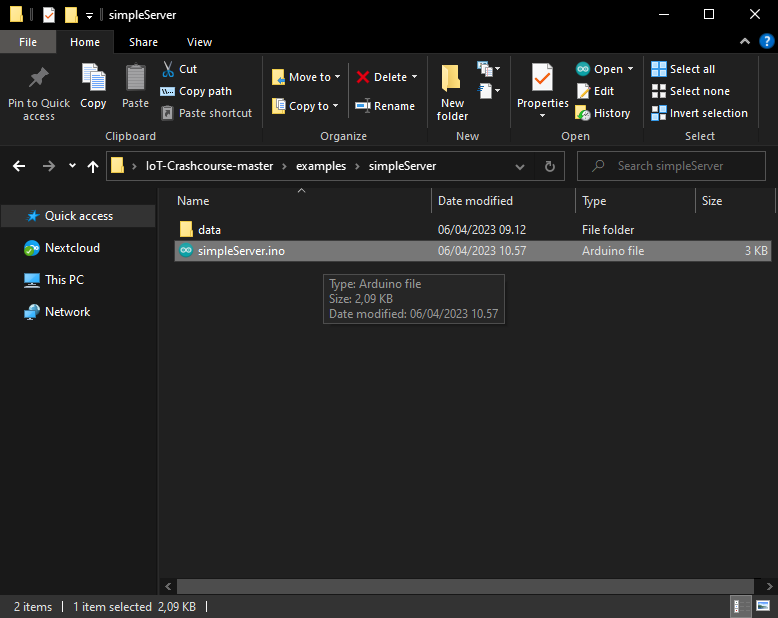
\includegraphics[height=0.6\textheight,keepaspectratio=true]{assets/pictures/examplefolder.png}
  			\caption{Åbnet folder for "\tthigh{simpleServer}" et af eksemplerne. .ino filen indeholder koden, og "\tthigh{data}" mappen ekstra filer, der skal lægges på ESP32 boardet}
  			\label{fig:examplefolder}
		\end{figure}
	\end{column}

	\begin{column}{0.5\textwidth}
		\begin{textBox}
			\begin{itemize}
				\item For at åbne en sketch (program), fra de inkluderede eksempler fra workshoppen:
				\begin{itemize}
					\item Åbn "\tthigh{examples}" folderen blandt de udpakkede filer
					\item Dernæst åbn sketch folderen (f.eks. "\tthigh{simpleServer}")
					\item Dobbeltklik på .ino filen
					\item Kan også kendes på dette ikon: (
\includegraphics[height=12pt, keepaspectratio=true]{assets/pictures/arduino-icon.png})
				\end{itemize}
			\end{itemize}
		\end{textBox}
	\end{column}
	
\end{columns}
\end{frame}

\begin{frame}{Åbning af sketch}
\begin{columns}

	\begin{column}{0.5\textwidth}
		\begin{textBox}
			\begin{itemize}
				\item Eksemplet i denne guide tager udgangspunkt i simpleServer
				\item Når sketchen er åbnet, skal to variable skiftes ud for at fungere:
				\begin{itemize}
					\item \tthigh{ssid} skal være et WiFi der er tilgængeligt, f.eks.: \tthigh{"mitHjemmeWiFi"}
					\item \tthigh{password} skal være passwordet til dette, f.eks.: \tthigh{"mitPassword123"}
					\begin{itemize}
						\item Hvis der ikke er noget password, skal det være tomt, dvs.: \tthigh{""}
					\end{itemize}
				\end{itemize}
			\end{itemize}
		\end{textBox}
	\end{column}

	\begin{column}{0.5\textwidth}
		\begin{figure}
  			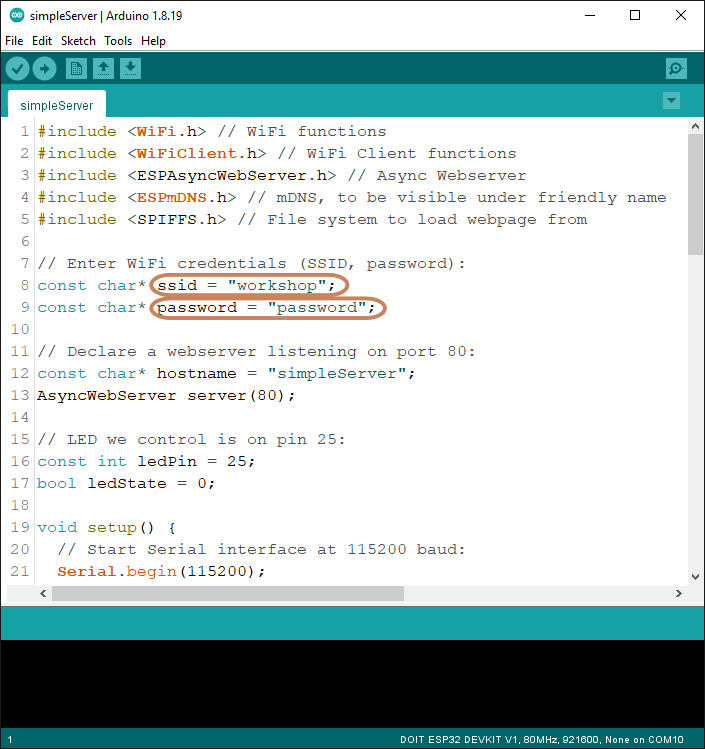
\includegraphics[height=0.6\textheight,keepaspectratio=true]{assets/pictures/simpleServer.png}
  			\caption{\tthigh{simpleServer} eksemplet indlæst i Arduino IDE. \tthigh{ssid} og \tthigh{password} skal indstilles til et tilgængelig WiFi-forbindelse}
  			\label{fig:simpleServer}
		\end{figure}
	\end{column}
	
\end{columns}
\end{frame}

\subsection{Upload trin}
\begin{frame}{Upload trin}
\begin{columns}

	\begin{column}{0.5\textwidth}
		\begin{figure}
  			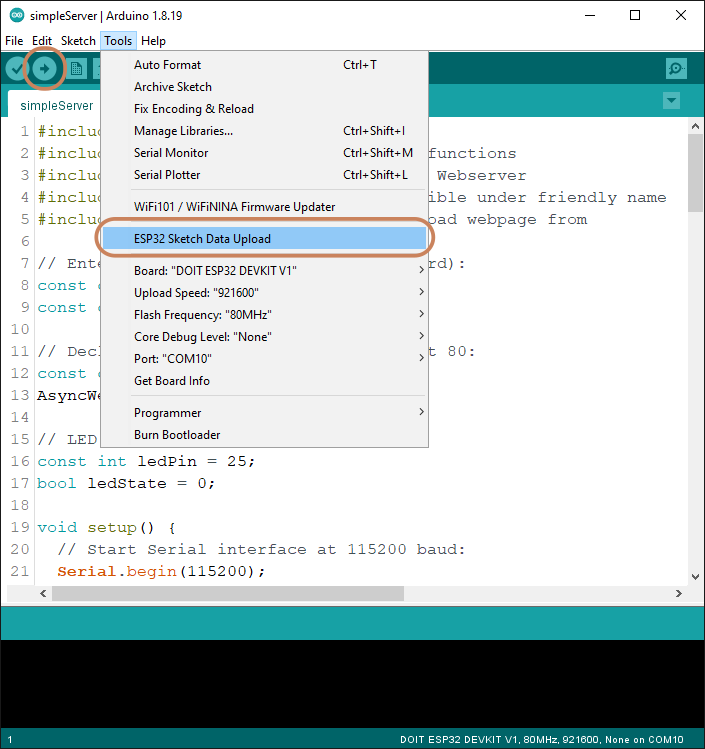
\includegraphics[height=0.6\textheight,keepaspectratio=true]{assets/pictures/ESP32-sketchdata-and-upload-marked.png}
  			\caption{Upload (\includesvg[height=8pt, keepaspectratio=true]{assets/svg/ide-upload.svg}) og "\tthigh{Tools} > \tthigh{ESP32 Sketch Data Upload}" markeret i Arduino IDE}
  			\label{fig:ESP32-sketchdata-and-upload-marked}
		\end{figure}
	\end{column}

	\begin{column}{0.5\textwidth}
		\begin{textBox}
			\begin{itemize}
				\item I mange sketches med ESP32 er der \tthigh{to} trin til at programmere sit board:
				\begin{enumerate}
					\item Upload af sketch
					\item Upload af ekstra Sketch data \\
					(Ligger i sketch folderen under mappen "\tthigh{data}")
				\end{enumerate}
				\item Det ordnes ved hhv.:
				\begin{enumerate}
					\item At trykke på Upload (\includesvg[height=12pt, keepaspectratio=true]{assets/svg/ide-upload.svg}) i IDE'et
					\item At trykke på "\tthigh{Tools} > \tthigh{ESP32 Sketch Data Upload}"
				\end{enumerate}
			\end{itemize}
		\end{textBox}
	\end{column}

\end{columns}
\end{frame}

\begin{frame}{Upload trin}
\begin{columns}

	\begin{column}{0.5\textwidth}
		\begin{textBox}
			\begin{itemize}
				\item Inden de førnævnte trin, skal boardet specificeres.
				\begin{itemize}
					\item For at uploade til ESP32 boardet, vælges "\tthigh{Board} > \tthigh{ESP32 Arduino} > \tthigh{DOIT ESP32 DEVKIT V1}"
					\item Resten af punkterne, som f.eks. Upload Speed, skal stå som vist.
				\end{itemize}
			\end{itemize}
		\end{textBox}
	\end{column}

	\begin{column}{0.5\textwidth}
		\begin{figure}
  			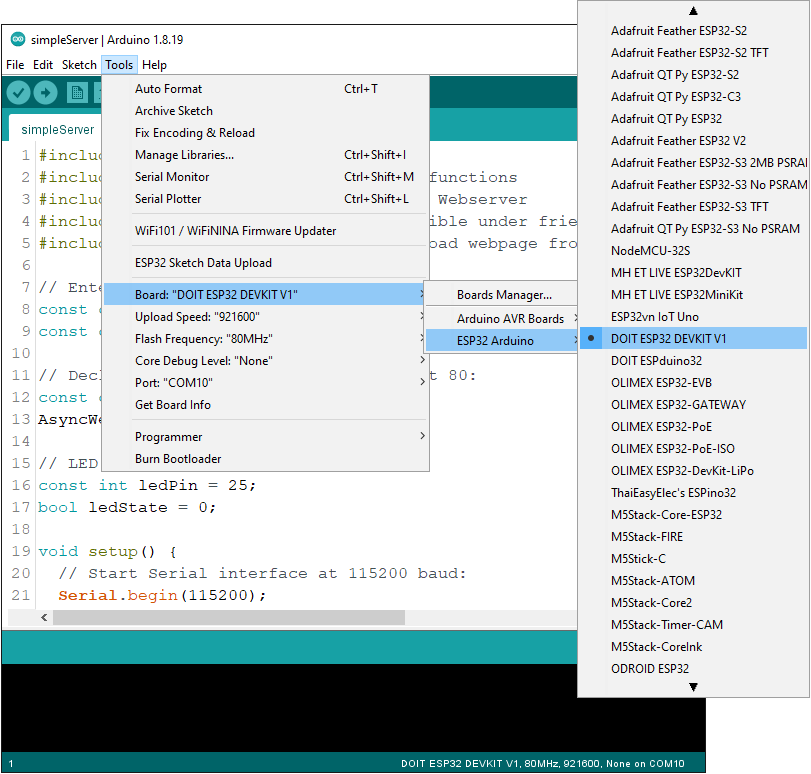
\includegraphics[height=0.6\textheight,keepaspectratio=true]{assets/pictures/boardselection.png}
  			\caption{Valg af boardet "\tthigh{Board} > \tthigh{ESP32 Arduino} > \tthigh{DOIT ESP32 DEVKIT V1}" i Arduino IDE}
  			\label{fig:boardselection}
		\end{figure}
	\end{column}

\end{columns}
\end{frame}

\begin{frame}{Upload trin}
\begin{columns}

	\begin{column}{0.5\textwidth}
		\begin{figure}
  			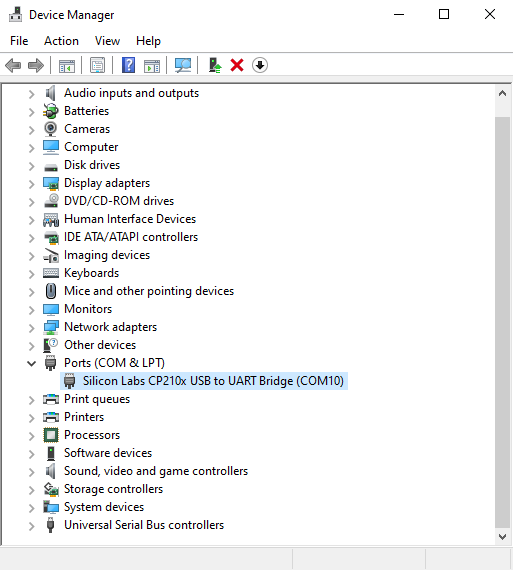
\includegraphics[height=0.6\textheight,keepaspectratio=true]{assets/pictures/devicemanager.png}
  			\caption{\tthigh{Silicon Labs CP210x USB to UART Bridge} vist i Windows Device Manager}
  			\label{fig:devicemanager}
		\end{figure}
	\end{column}

	\begin{column}{0.5\textwidth}
		\begin{textBox}
			\begin{itemize}
				\item Der skal også vælges hvilken kommunikationsport Arduino IDe bruger til upload
				\begin{itemize}
					\item På windows kan den ses under Windows-programmet "\tthigh{Device Manager}"
					\begin{itemize}
						\item ("\tthigh{Enhedshåndtering}" på dansk)
					\end{itemize}
					\item Under navnet "\tthigh{Silicon Labs CP210x USB to UART Bridge}"
					\begin{itemize}
						\item Denne enhed har porten \tthigh{COM10}
						\item \ttwarn{VIGTIGT}: Det ændrer sig ofte pga. tilgængelighed af portene, så vær opmærksom!
					\end{itemize}
				\end{itemize}
			\end{itemize}
		\end{textBox}
	\end{column}

\end{columns}
\end{frame}

\begin{frame}{Upload trin}
\begin{columns}

	\begin{column}{0.5\textwidth}
		\begin{textBox}
			\begin{itemize}
				\item Porten vælges på listen over porte i Arduino IDE: "\tthigh{Tools} > \tthigh{Port}"
				\begin{itemize}
					\item I dette tilfælde COM10
				\end{itemize}								
			\end{itemize}
		\end{textBox}
	\end{column}
	
	\begin{column}{0.5\textwidth}
		\begin{figure}
  			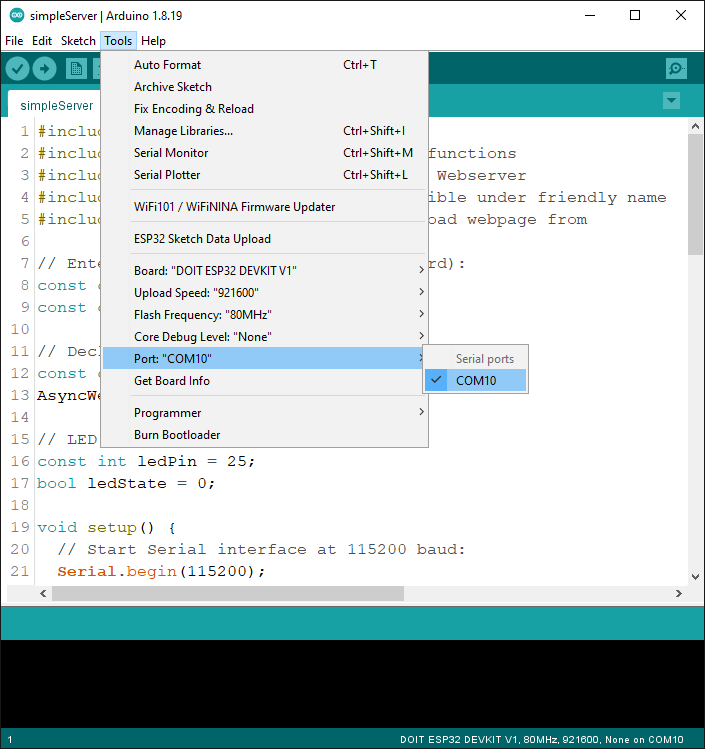
\includegraphics[height=0.6\textheight,keepaspectratio=true]{assets/pictures/comport.png}
  			\caption{COM-porten COM10 valgt under "\tthigh{Tools} > \tthigh{Port}"}
  			\label{fig:comport}
		\end{figure}
	\end{column}

\end{columns}
\end{frame}

\begin{frame}{Upload trin}
\begin{columns}

	\begin{column}{0.5\textwidth}
		\begin{figure}
  			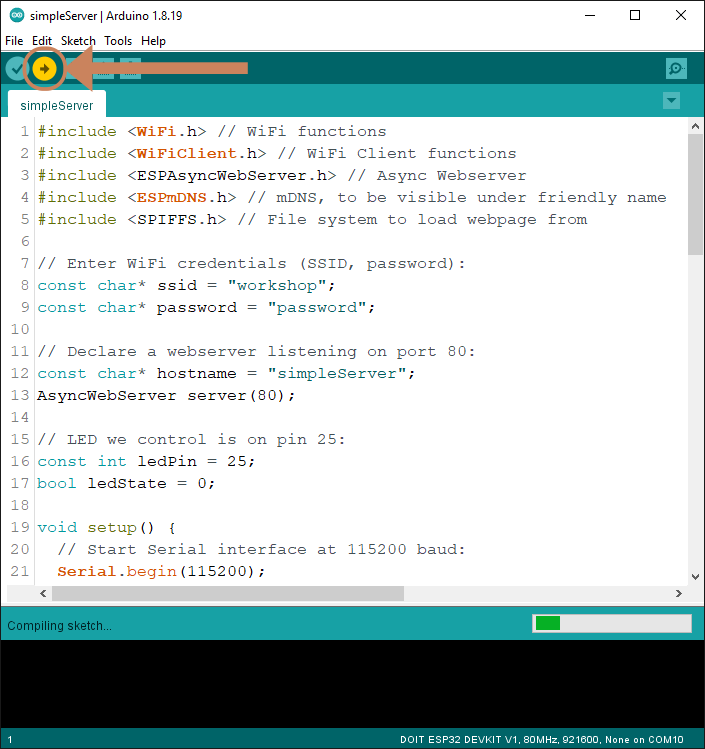
\includegraphics[height=0.6\textheight,keepaspectratio=true]{assets/pictures/compilingsketch.png}
  			\caption{Igangsat kompilering og upload i Arduino IDE}
  			\label{fig:compilingsketch}
		\end{figure}
	\end{column}

	\begin{column}{0.5\textwidth}
		\begin{textBox}
			\begin{itemize}
				\item Herefter trykkes på Upload (\includesvg[height=12pt, keepaspectratio=true]{assets/svg/ide-upload.svg})
				\begin{itemize}
					\item Sketchen vil kompilere og derefter uploades til det valgte board over COM-porten
					\item Det kan tage lidt tid
				\end{itemize}
			\end{itemize}
		\end{textBox}
	\end{column}
	
\end{columns}
\end{frame}

\begin{frame}{Upload trin}
\begin{columns}

	\begin{column}{0.5\textwidth}
		\begin{textBox}
			\begin{itemize}
				\item Når der står "\tthigh{Done Uploading}", samt "\tthigh{Hard resetting via RTS pin}" i uploaddialogen nederst, er boardet færdigt med første upload
			\end{itemize}
		\end{textBox}
	\end{column}
	
	\begin{column}{0.5\textwidth}
		\begin{figure}
  			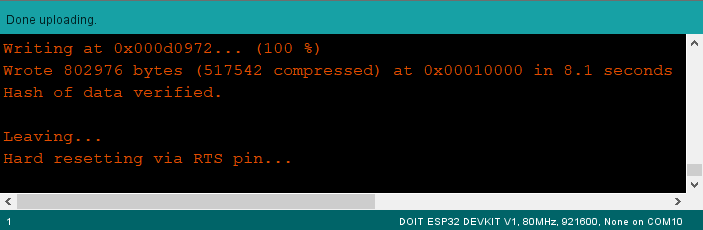
\includegraphics[width=\textwidth,keepaspectratio=true]{assets/pictures/doneuploading.png}
  			\caption{Uploaddialogen i Arduino IDE efter et succesfuldt upload}
  			\label{fig:doneuploading}
		\end{figure}
	\end{column}
	
\end{columns}
\end{frame}

\begin{frame}{Upload trin}
\begin{columns}

	\begin{column}{0.5\textwidth}
		\begin{figure}
  			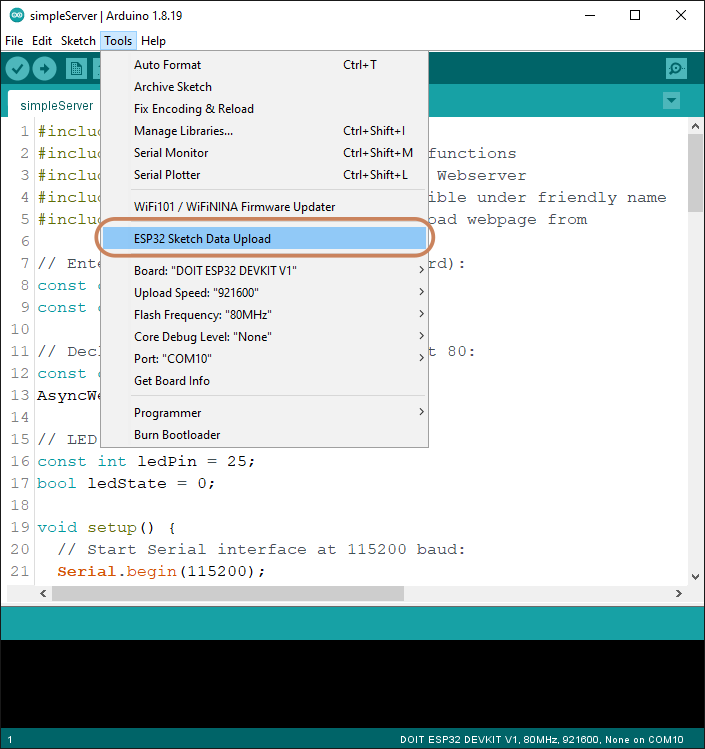
\includegraphics[height=0.6\textheight,keepaspectratio=true]{assets/pictures/ESP32-sketchdata-marked.png}
  			\caption{"\tthigh{Tools} > \tthigh{ESP32 Sketch Data Upload}" i Arduino IDE}
  			\label{fig:ESP32-sketchdata-marked}
		\end{figure}
	\end{column}

	\begin{column}{0.5\textwidth}
		\begin{textBox}
			\begin{itemize}
				\item Herefter udføres et evt. Sketch Data Upload, hvis sketchen inderholder en "\tthigh{data}" mappe
				\begin{itemize}
					\item Tryk på "\tthigh{Tools} > \tthigh{ESP32 Sketch Data Upload}"
					\item \ttwarn{VIGTIGT}: Hvis et "Serial Monitor" vindue er åbent, fungerer Sketch Data Upload ikke
				\end{itemize}
			\end{itemize}
		\end{textBox}
	\end{column}

\end{columns}
\end{frame}

\begin{frame}{Upload trin}
\begin{columns}
	\begin{column}{0.5\textwidth}
		\begin{textBox}
			\begin{itemize}
				\item Når der står "\tthigh{SPIFFS Image Uploaded}", samt "\tthigh{Hard resetting via RTS pin}" i uploaddialogen nederst, er boardet færdigt med andet upload
			\end{itemize}
		\end{textBox}
	\end{column}
	
	\begin{column}{0.5\textwidth}
		\begin{figure}
  			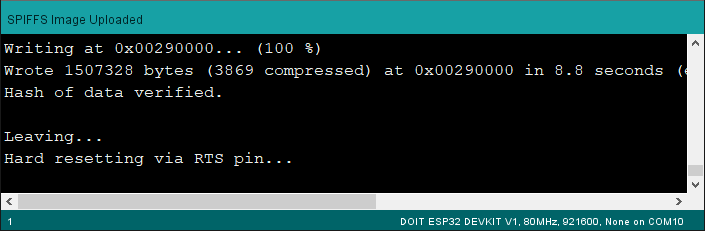
\includegraphics[width=\textwidth,keepaspectratio=true]{assets/pictures/sketchdatauploaded.png}
  			\caption{Uploaddialogen i Arduino IDE efter et succesfuldt Sketch Data upload}
  			\label{fig:sketchdatauploaded}
		\end{figure}
	\end{column}

\end{columns}
\end{frame}

\subsection{Test af uploadet kode}
\begin{frame}{Test af uploadet kode}
\begin{columns}

	\begin{column}{0.5\textwidth}
		\begin{figure}
  			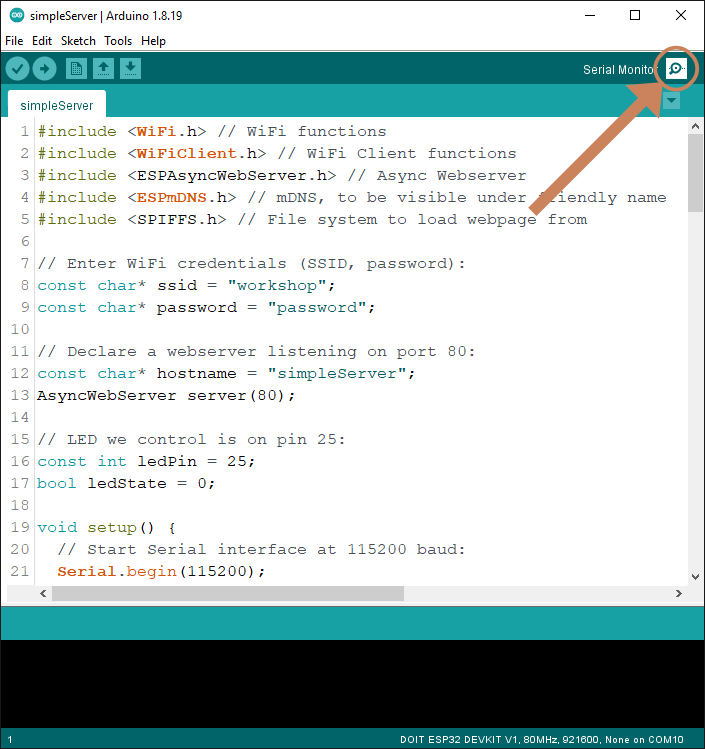
\includegraphics[height=0.6\textheight,keepaspectratio=true]{assets/pictures/serial-monitor.png}
  			\caption{Serial Monitor (\includesvg[height=8pt, keepaspectratio=true]{assets/svg/ide-serial.svg}) markeret i Arduino IDE}
  			\label{fig:serial-monitor}
		\end{figure}
	\end{column}
	
	\begin{column}{0.5\textwidth}
		\begin{textBox}
			\begin{itemize}
				\item For at tjekke om alt kører som det skal, kan man klikke på Serial Monitor (\includesvg[height=12pt, keepaspectratio=true]{assets/svg/ide-serial.svg}) i øverste højre hjørne
				\begin{itemize}
					\item Dette åbner \tthigh{Serial Monitor} vinduet, som er kommunikation til/fra boardet
					\item \ttwarn{VIGTIGT}: Hvis et "Serial Monitor" vindue er åbent, fungerer Sketch Data Upload ikke
				\end{itemize}
			\end{itemize}
		\end{textBox}
	\end{column}

\end{columns}
\end{frame}

\begin{frame}{Test af uploadet kode}
\begin{columns}
	
	\begin{column}{0.5\textwidth}
		\begin{textBox}
			\begin{itemize}
				\item Indstil Serial Monitor vinduet til \tthigh{115200 baud}, da sketchen bruger denne kommunikationshastighed, og ESP32's diagnostik også gør
				\begin{itemize}
					\item Ellers vil der formentlig stå "⸮⸮⸮⸮⸮⸮" eller tilsvarende volapyk i vinduet
					\item Indstillingen findes i bunden af vinduet
				\end{itemize}
			\end{itemize}
		\end{textBox}
	\end{column}
	
	\begin{column}{0.5\textwidth}
		\begin{figure}
  			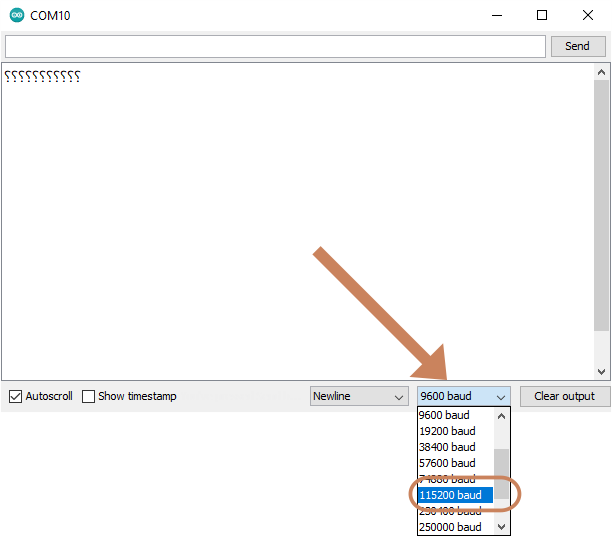
\includegraphics[height=0.6\textheight,keepaspectratio=true]{assets/pictures/serial-monitor-115200-baud.png}
  			\caption{Serial Monitoren indstillet til \tthigh{115200 baud} (tegn i sekundet) for at tyde teksten fra ESP32}
  			\label{fig:serial-monitor-115200-baud}
		\end{figure}
	\end{column}

\end{columns}
\end{frame}

\begin{frame}{Test af uploadet kode}
\begin{columns}

	\begin{column}{0.5\textwidth}
		\begin{figure}
			\begin{columns}
				\begin{column}{0.2\textwidth}
  					\includesvg[height=0.6\textheight,keepaspectratio=true]{assets/svg/ESP32-EN-button.svg}
				\end{column}
				\begin{column}{0.7\textwidth}
  					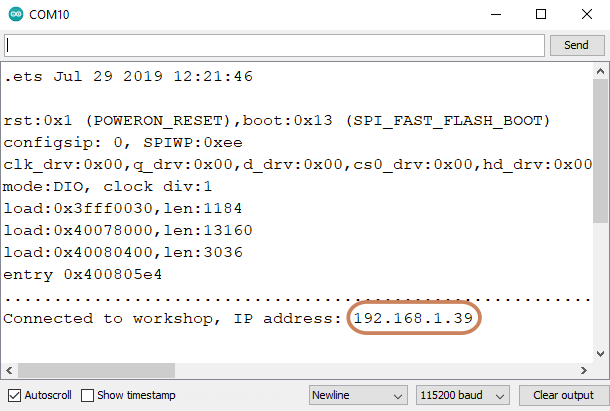
\includegraphics[width=\textwidth,keepaspectratio=true]{assets/pictures/connected.png}
				\end{column}
			\end{columns}
			\caption{Ved tryk på boardets EN knap, genstarter boardet, forbinder sig til WiFi, og outputter IP adressen den har fået}
  			\label{fig:connected}
		\end{figure}
	\end{column}
	
	\begin{column}{0.5\textwidth}
		\begin{textBox}
			\begin{itemize}
				\item Tryk på boardets "EN" knap for at genstarte det
				\item Hvis den har forbundet sig til et WiFi som i eksemplet med simpleServer, vil der stå en \tthigh{IP adresse} i Serial Monitor
				\begin{itemize}
					\item Hvis ESP32'eren siger "..." uendeligt, kan det skyldes manglende eller forkert "\tthigh{ssid}" og/eller "\tthigh{password}" i sketchen
					\item Disse kan ændres til at matche f.eks. et tilgængeligt hjemme-WiFi, som man kender navn og kodeord til
				\end{itemize}
			\end{itemize}
		\end{textBox}
	\end{column}
	
\end{columns}
\end{frame}

\begin{frame}{Test af uploadet kode}
\begin{columns}

	\begin{column}{0.5\textwidth}
		\begin{textBox}
			\begin{itemize}
				\item Indsæt den aflæste \tthigh{IP adresse} i en webbrowser
				\item Hvis alt er gået rigtigt, viser den simpleServer eksemplet
				\begin{itemize}
					\item Hvis siden indlæser uden at vise noget, eller giver fejl, kan det skyldes manglende "\tthigh{ESP32 Sketch Data Upload}", som nævnt tidligere
				\end{itemize}
			\end{itemize}
		\end{textBox}
	\end{column}

	\begin{column}{0.5\textwidth}
		\begin{figure}
  			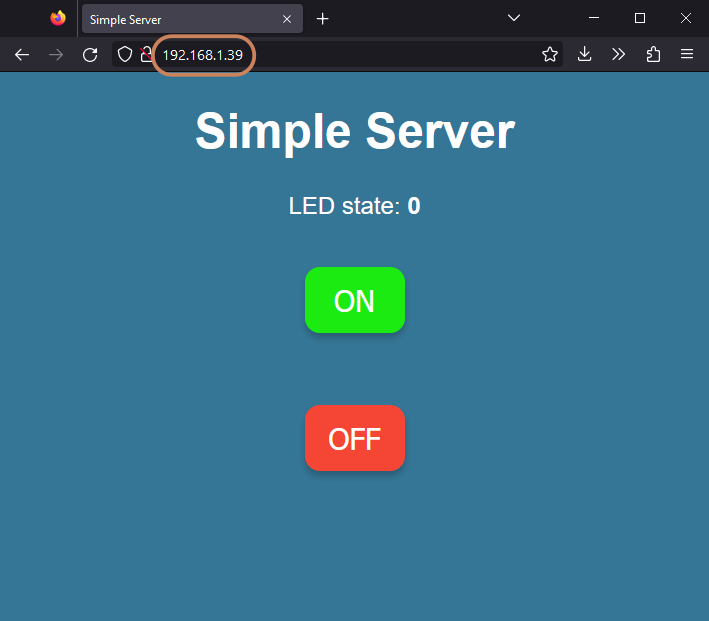
\includegraphics[height=0.6\textheight,keepaspectratio=true]{assets/pictures/visit-page.png}
  			\caption{\tthigh{simpleServer} eksemplet indlæst på Firefox webbrowseren via IP-adressen}
  			\label{fig:visit-page}
		\end{figure}
	\end{column}
	
\end{columns}
\end{frame}


\end{document}